At the backbone of all classical protocols described in Section \ref{section:protocols}, it lies the need to generate random uniform distributions of either qubit states, Bloch vectors or shared randomness in $\mathbb{R^3}$. In Figure \ref{fig:results_random_states}, we can see that applying random unitary transformations to zero qubit states leads to uniformly distributed random qubit pure states, which can later be transformed into random Bloch vectors or normalized random vectors in $\mathbb{R^3}$ as needed. These random states are also the seed to compute random POVMs with rank-1 projectors, as described in Section \ref{section:povm_generation}.
\begin{figure}[h]
\centering
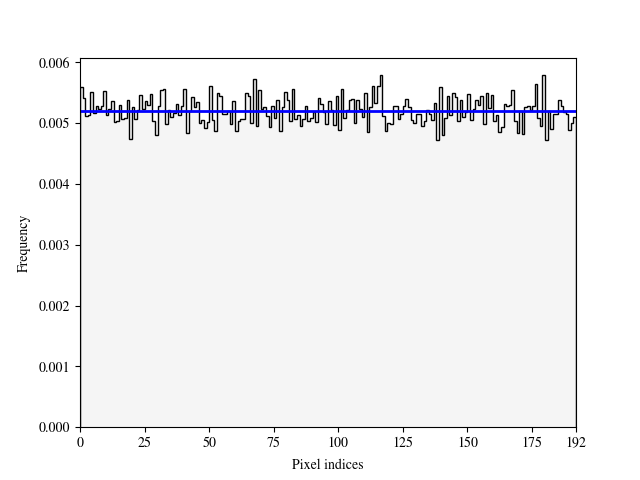
\includegraphics[width=\textwidth]{images/random_bloch_healpix.png}
\caption{In this histogram we see how the frequency distribution of $N=10^4$ random qubit states generated with \cite{software2023} follows a random uniform distribution of state vectors along the Bloch sphere (blue solid line). The frequencies are binned by HEALPix indices corresponding to an equal-area iso-latitude partition of the Bloch sphere with resolution $\mathit{NSIDE}=4$.}
\label{fig:results_random_states}
\end{figure}

Once we have proven to have means to generate random states and rank-1 POVMs, we can focus on the measurement process. The outcome probabilities for a given random POVM measure can be obtained analytically using the Born's rule, but we have gone a step further and used quantum simulators and noisy intermediate scale quantum computers to calculate such probabilities and compare them to the theoretical ones. For such purpose we have made an extensive use of Qiskit \href{https://qiskit.org/}{Qiskit} and \href{https://quantum-computing.ibm.com}{IBM Quantum}.

\textit{To be included:}

\textit{Quantum Simulator vs. NISQ Computer benchmarking}

\textit{Convergence plots, classical vs. quantum vs. theoretical probabilities}

\textit{Kullback-Leibler divergence plots}

\textit{Bell scenario joint probabilities convergence}

\textit{CHSH inequality}